%%%%%%%%%%%%%%%%%%%%%%%%%%%%%%%%%%%%%%%%%%%%%%%%%%%%%%%%%%%%%%%%%%%
%                                                                 %
%                            CHAPTER TWO                          %
%                                                                 %
%%%%%%%%%%%%%%%%%%%%%%%%%%%%%%%%%%%%%%%%%%%%%%%%%%%%%%%%%%%%%%%%%%%
\chapter{RELATED WORKS} \label{sec:related}
%talk about the main topic of your thesis, and a blurb about what is related

Sketch interpretation on a computer interface is not trivial to implement. While recording user input is not difficult, it is challenging to interpret the user's intent correctly. Drawings and sketches created by users are often ambiguous and difficult to understand for an application. The minute differences between user actions can result in the system returning vastly different outcomes. Higher degrees of accuracy often require large amounts of data, demanding higher computer specifications to execute properly. With greater resources demanded, it becomes increasingly difficult for sketch interpretation to become available for widespread use. \\

% This thesis provides an alternative sketching interface for the online architectural sketching interface for simulations (OASIS). The OASIS is an architectural sketching application designed for early design prototyping \cite{oasis2016}. Using OASIS, users can create daylight simulations based on user-designed models. 

In this chapter, I will outline some work done on OASIS prior to the development of this sketching interface. We will also discuss some related works regarding sketch recognition, and its applicability to this application. Finally, we discuss some related software and their approaches to reaching similar goals.

%PICTURES OF OASIS
%PICTURES OF OASIS
%PICTURES OF OASIS

\section{OASIS}

OASIS is an online architectural sketching application developed by fellow colleague, Max Espinoza \cite{oasis2016}. Its primary purpose is to generate closed 3D meshes with optimal properties for simulations. OASIS is an alternative form of the Virtual Heliodon, a tangible user interface for daylighting simulation \cite{yusheng}.  Currently, OASIS only supports simulating daylight visualizations \cite{oasis2016}. To begin, users create 2D floor plans using the design interface. Next, OASIS interprets and constructs 3D models based on the designs. Finally, the tasks may be generated with various parameters and executed on one of our servers.

\begin{figure}[ht]
\centering
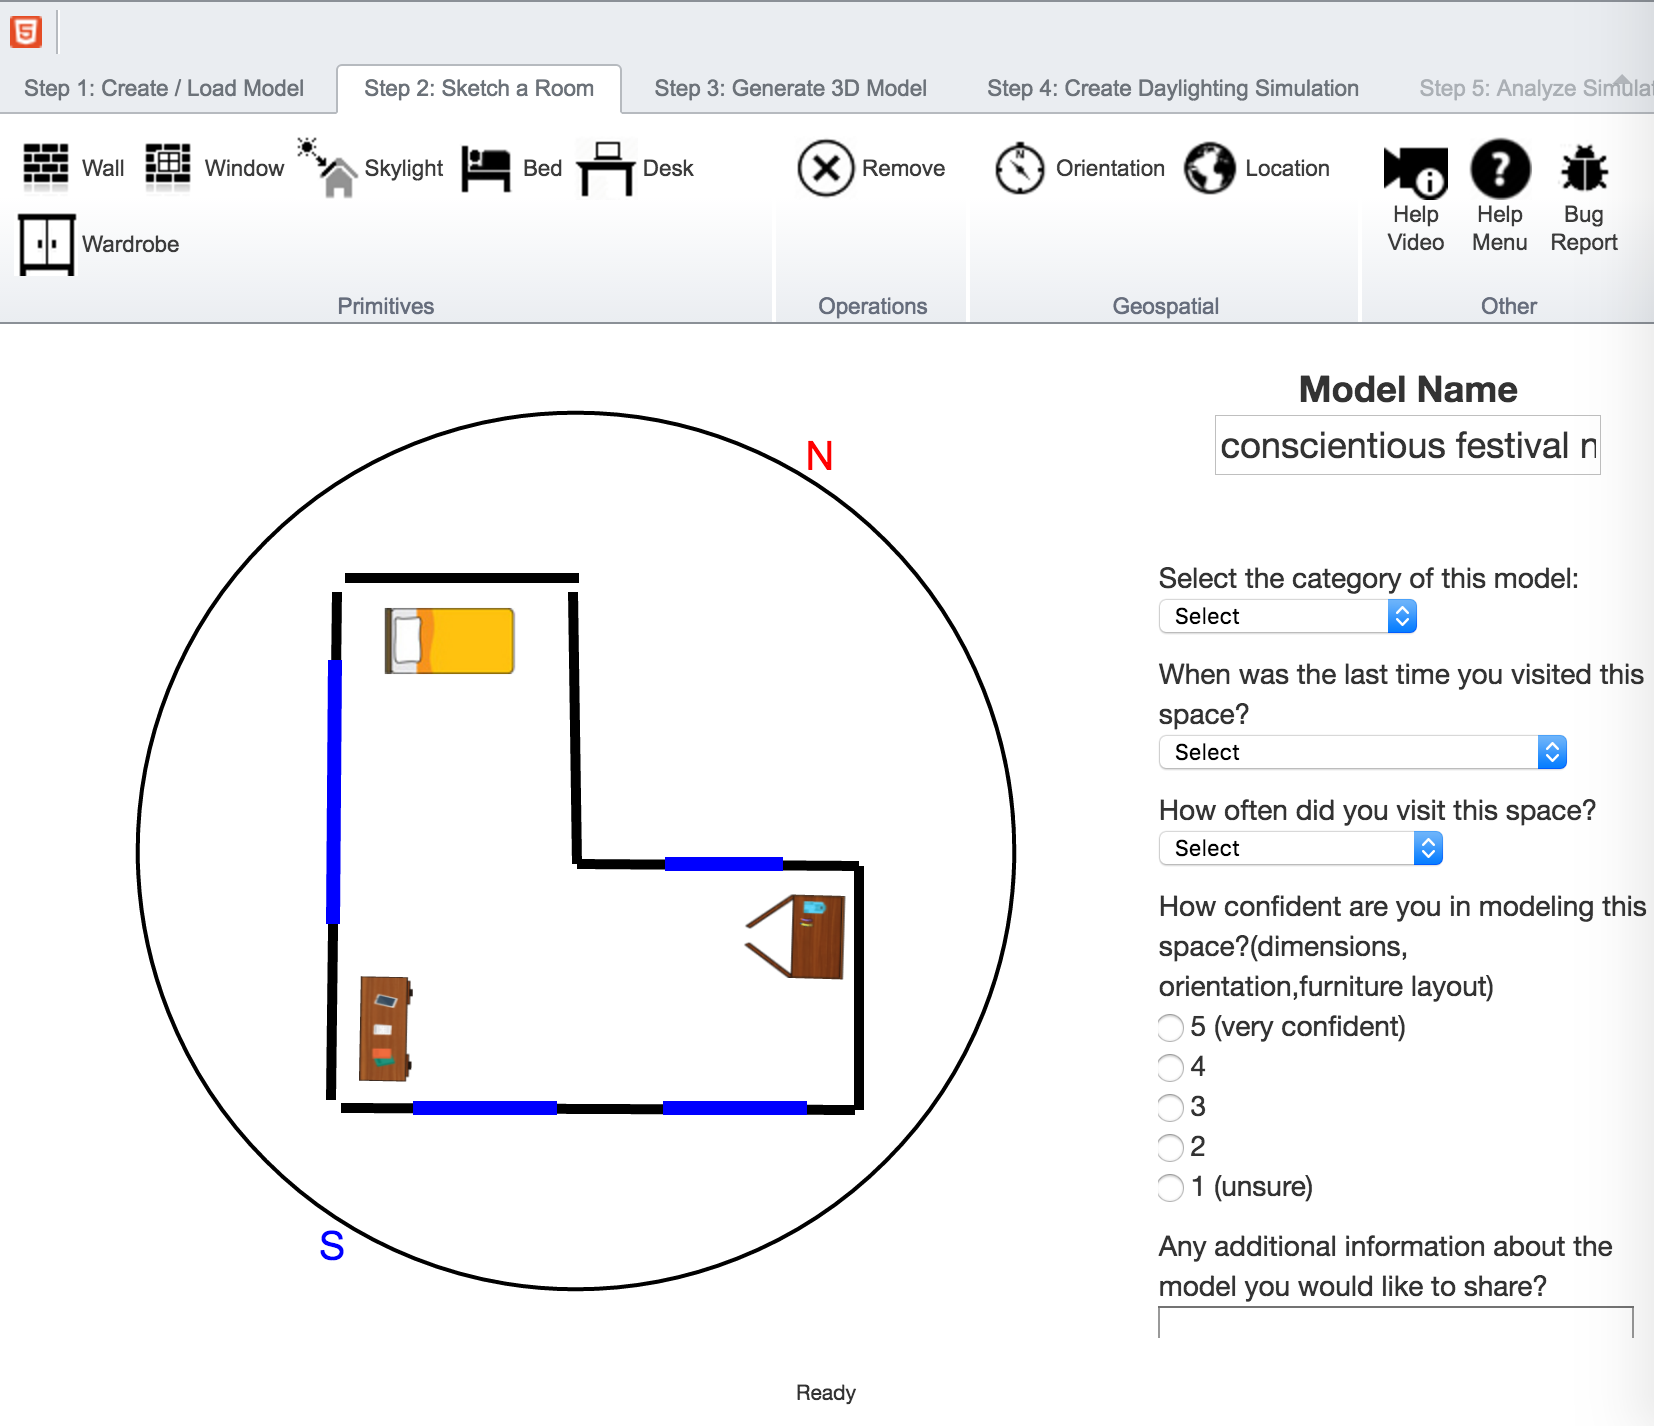
\includegraphics[width=\textwidth]{oasis}
\caption[Image of the sketching interface used in OASIS]{Image of the sketching interface used in OASIS \cite{oasis2016}.}
\label{fig:oasis}
\end{figure}

There are many design choices available when creating a sketch on OASIS. Users can create walls, windows, beds, desks, and wardrobes. All furniture items are editable and easily configurable. Along with basic primitives, a cardinal orientation for the room may be chosen, as well as any location in the world. When creating daylighting tasks, users have options when simulating the environment surrounding their rooms. Tasks are editable with dates, times, timezones, and weather condition. Users also have the option to share their models with others via URL \cite{oasis2016}. A unique link can be shared with family and friends to show off designs and gather feedback. Overall, OASIS provides a wide array of choices for users to personalize their designs.

\section{Previous Work on OASIS}

My contributions to OASIS are not limited to the creation of the new sketching interface. Before the inception of this work, I developed features and fixed bugs to improve user experience on OASIS. The time spent improving the application was invaluable for gaining familiarity with the system and learning about the development process. Using OASIS also helped me realize some of its flaws, which helped inspire the creation of this thesis. Without this prior experience, developing a new sketching interface would have been far more difficult. \\

One contribution was the implementation of a Cron job to regularly select tasks. Cron is a time based scheduler in Unix-based systems that runs commands at preset intervals \cite{cron}. The implemented Cron job is set to check user submissions at short intervals for newly submitted tasks, and execute them using the daylight simulation rendering engine. Before the implementation of the Cron job, there was no method to select one task over another task, and tasks were run when they were submitted. This could cause problems overloading the server if too many tasks were queued at the same time. The importance of the Cron job is to give the system control over which task will be processed next. Currently, the script selects based on first-come-first-serve. However, the selection process could be improved in the future to increase fairness between users. For example, if a User A enters the queue while User B has 100 tasks already in queue, it would be unfair for User A's task to be the 101st task processed, even if it was the 101st task created. \\

The task tab is where the user can create daylighting simulation tasks for our server to process. I made a number of improvements to the task tab to improve user experience, including dynamic sizing of the table, additional information about the tasks themselves, improved readability, and automatic timezone estimation. Timezone estimation is based on the user's choice of location when designing using the sketching interface. Based on the x and y coordinates of the location selection, I estimate which timezone it is closest to, and automatically select that timezone when a user creates a new task. \\

In daylighting simulations, the importance of windows cannot be understated, since the illumination of the room is entirely based on windows. Consequently, there is a high priority for windows to be designed correctly. One enhancement to the old sketching interface composed primarily of improved window snapping. In OASIS, windows are created by switching into window mode and drawing a stroke near a wall, snapping the window directly onto the wall. There existed minor issues involving the creation of walls with zero or infinite slope. If a user created a window and attached it to a wall with a zero or infinite slope, the window would snap to the maximum length of the wall, regardless of its intended length. The behavior for wall snapping was improved to attach only to the nearest wall with a relatively similar slope to the window drawn, with a maximum length of 90 percent of the wall (5 percent extra room on both ends), and to snap a window of the user's intended length regardless of the slope of the wall. This wall creation procedure heavily influenced the creation of windows in the new sketching interface. \\

\begin{figure}[ht]
\centering
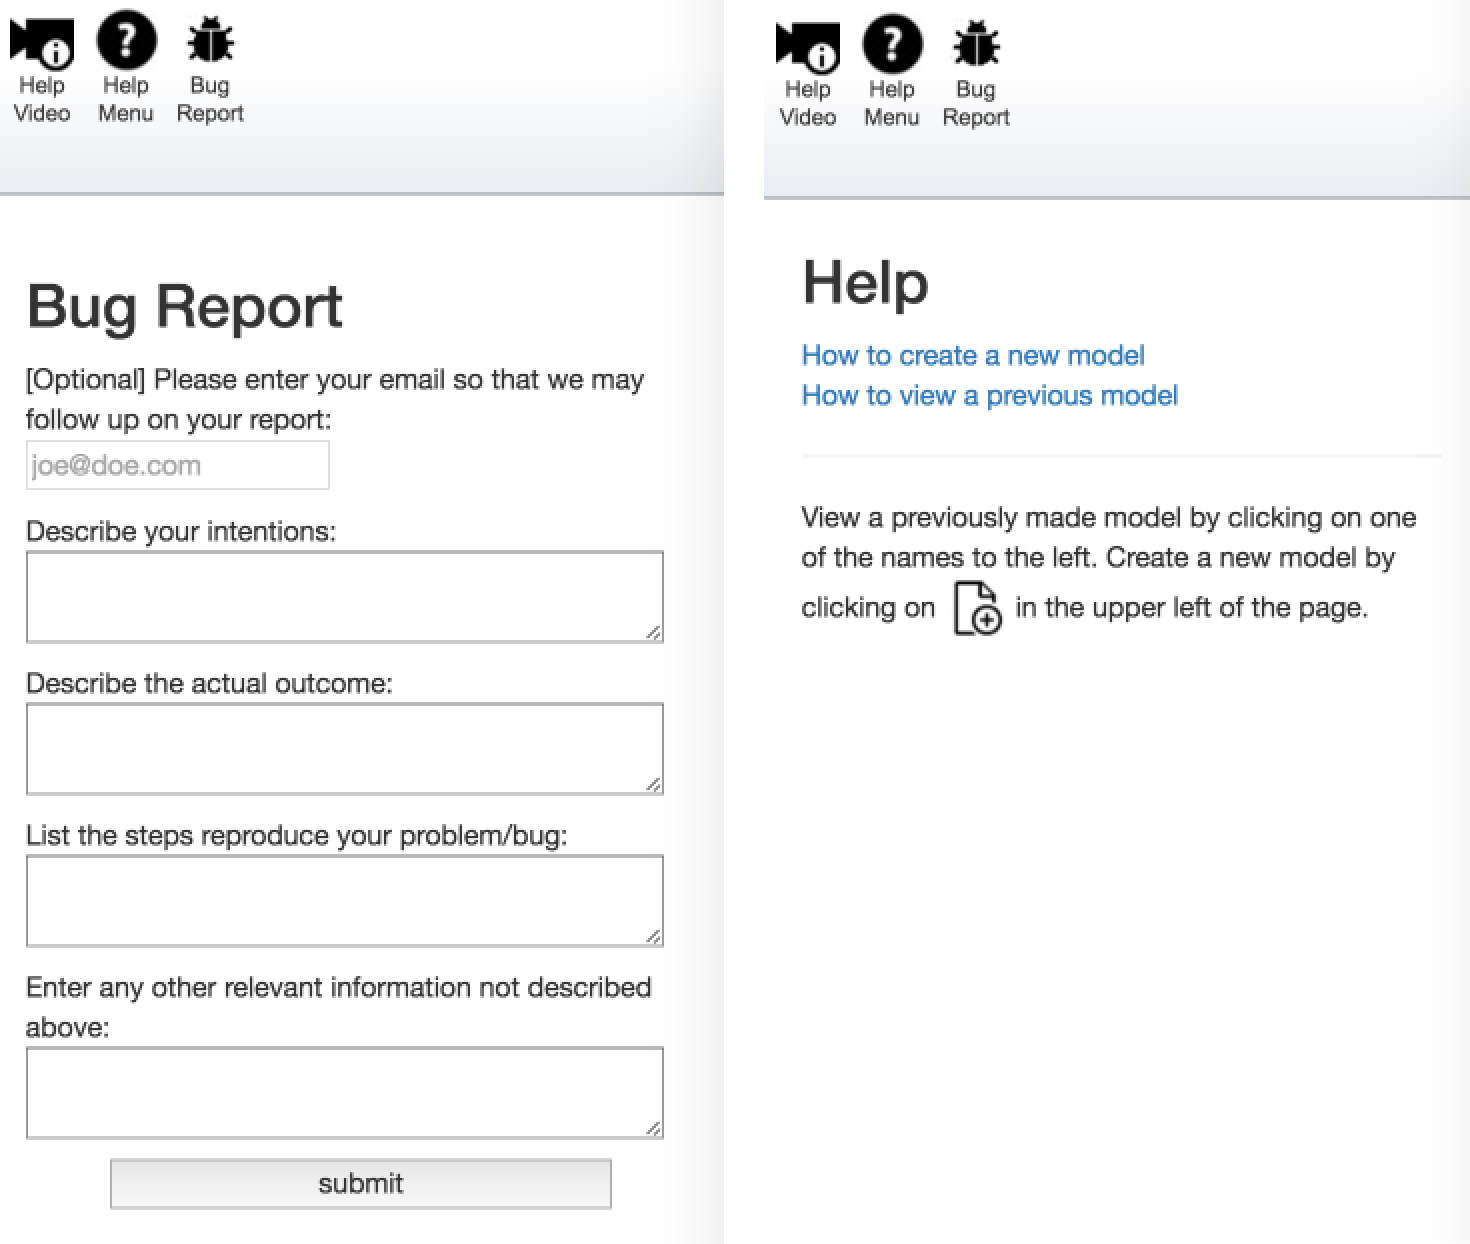
\includegraphics[width=.75\textwidth]{newmenus}
\caption[OASIS bug report and help menu additions]{Left: Bug report submission menu. Right: Help menu with directions based on page.}
\label{fig:newmenus}
\end{figure}

During some initial user tests, users found it difficult to find help on what to do, or how to do something. At the same time, we realized it was difficult to replicate and fix problems described by users in the user feedback section. Our attempt at solving these problems was the implementation of the help and bug report menus. These menus, when selected, would replace the space previous occupied by user feedback. The bug report menu allowed users to submit bug reports to the developers to improve the website. As shown in Figure \ref{fig:newmenus}, information submitted included the intent of the user and methods of reproduction. Using the information acquired, the goal would be improving the quality of the site and reducing the number of bugs users encountered. The help menu included information based on what page the user was browsing, and included animated gifs to display what actions needed to be done.  \\

OASIS is in a state of constant development and improvement, with help from a team of dedicated developers and users. From the enhancements listed in this section, the number of bugs has decreased while the quality of user experience increased. Using the knowledge gained from prior improvements, I applied the same concepts in creating this thesis work. \\

\section{Stroke Recognition}

Since the user's only input into the sketching interface is a series of recorded gestures, some method of interpreting those actions is necessary. Recognizing gestures is difficult because the system needs to recognize that different inputs can often have the same or similar meaning. The amount of variability in a gesture or stroke is sometimes difficult to account for and sometimes the smallest inconsistency can create a wildly different classification. At the same time, the opposite may also be true; an extra action at the end of a gesture may be the defining difference between two classifications. \\

\subsection{Human Input Recognition}
%talk about the difficulty of human input, bring up an example
One example of the difficulty of recognizing human input is reading human handwriting. The variability in each person's style of writing produces a problem where infinitely many inputs may imply the same meaning, as exampled in Figure \ref{fig:handwriting}. According to a survey conducted by Plamondon and Srihari, the inputs to handwriting systems are often separated into two groups: online and offline \cite{handwritingrec}. Online recognition involves user input being captured by a computer interface, as a representation of time, order, and points. For example, the NPen++ online handwriting recognizer collects up to 200 points per second, based on the user's pen input using a Wacom tablet \cite{npen}. Offline recognition refers to a user writing on a physical surface, and that information being scanned and  digitally processed. While online recognition is typically faster and more accurate due to more information being collected \cite{neural2011}, the offline recognition of physical handwriting recognition cannot be ignored, due to its prevalence in everyday life \cite{handwritingrec}. This thesis work uses solely online recognition, as the architectural sketching interface is built on the web for maximum availability to users everywhere.

\begin{figure}[ht]
\centering
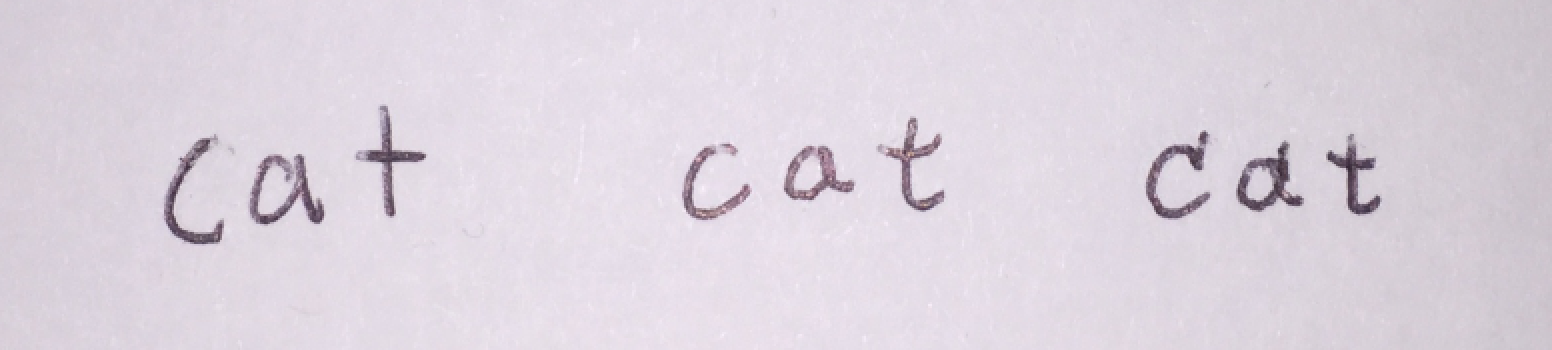
\includegraphics[width=.75\textwidth]{catwriting}
\caption[Examples of handwriting variations]{Above is an example of how three writings of the same word, even by the same person, can look different and contain the same meaning.}
\label{fig:handwriting}
\end{figure}

The use of machine learning has been extremely prevalent in human input recognition due to its high accuracy. Many types of machine learning algorithms have been employed to recognize human handwriting, such as hidden Markov models \cite{hmm1994} and neural networks \cite{neural2011}. However, the main drawback of machine learning based approaches is that they all require a large amount of data. In order to learn the finer details between different inputs, a learning algorithm must process a considerable amount of training data before it is effective. For example, the NPen++ recognizer uses a training set of roughly 13,000 words \cite{npen}, while the IAM English sentence database for handwriting recognition contains over 80,000 samples \cite{iamdatabase}. In this work, we choose to take a geometric approach to recognizing user input. While it may be less accurate and less flexible, a geometric approach allows for a faster implementation and tighter control on acceptable input. \\

\subsection{Other Recognizers}

While one recognizer was used most prominently, two other recognizers were also researched. One was a fuzzy recognizer developed by Fonseca and Jorge \cite{fuzzylogic}. This fuzzy logic based recognizer first created strokes (a series of points) and shapes (a recognized stroke), and computed a number of geometric features based on each strokes. Using the features extracted, Fonseca and Jorge created rules, along with allowable percentiles to determine the identity of a stroke. For example, to assist in identifying a circle, they used a \textit{thinness} ratio, which is defined as the perimeter square divided by the area of the convex hull. For different shapes, the allowed values for each of the ratios differed. When a user entered a stroke, the features would be extracted, and ratios calculated. Based on the ratios, a likely candidate could be chosen. Possible classifications included arrows, squares, rectangles, triangles, and circles. \\

While the accuracy of the implementation was high (over 90 percent successfully recognized \cite{fuzzylogic}), and the design was simple to understand and implement, a few factors led me to not pursue this any further. The implementation seemed to require heavy micromanagement of ratios. The implementation did not offer any methods of calculating the cutoffs using training data, leaving me to infer the adjustments were made by hand. While it appeared to work very well on geometric shapes, I had a difficult time recreating the process well on symbols such as letters of the alphabet. The metrics work well on simply defined user input such as as square or triangle, and it worked well on simple letters such as `C` or `T`, but I found it difficult to mathematically define more complex letters such as `B` or `Q`. When creating this application, the initial idea was to classify objects using letters as identifiers. Without a confident method of identifying letters, I felt I could not proceed at the time. Overall the fuzzy logic recognizer was intriguing and promising but did not fit my goals and purposes. \\

Another recognizer researched was a HMM machine learning based recognizer created by Hu \textit{et. al} \cite{hmm1994}. This recognizer used a      `left-to-right` hidden Markov model to score features such as  stroke tangents, translation, rotation, and scaling. A hidden Markov model is a model in which the system being modeled is assumed to be a Markov process with hidden states. A Markov process is one that satisfies the Markov property, which states that all states of the process are based solely on the current state. In this recognizer, each letter is broken down into segments, and recognized afterwards. This implementation describes an approach using \textit{nebulous stroke models}, which they do not define the letters or any features of letters, or how they are segmented. The program itself defines the most natural way of defining a letter. The models are trained using a 3 step process: letter training, linear word training, and lattice word training. Letter training involves training the system on single letters, linear word training uses whole words, and lattice word training transforms all words into finite state networks, and the system is trained on those. \\ 

Overall the hidden Markov model based approach was well defined, but it was overly complicated for my needs. If I had used this approach, a vast majority of my time would have been spent implementing and refining the recognizer into my system instead of developing an interface for OASIS. My primary goal, first and foremost, was to develop a sketch-based interface for OASIS, and not necessarily develop a unique recognizer.

\subsection{\$N Recognizer}
%$N, $1, explain in detail
One recognizer that I tested and used extensively was the \$N recognizer. There existed a few reasons for initially relying heavily on this recognizer for recognizing nearly everything in the system. One, the recognizer was simple to implement and modify. Second, the system was flexible in its ability to recognize both shapes and letters. Lastly, it did not require any training data, so the addition of new recognizable symbols was effortless. \\

The \$N is a lightweight, concise multistroke recognizer that generalizes one multistroke to all possible multistrokes \cite{dollarN}. To understand the \$N recognizer, we must first review its predecessor, the \$1 recognizer for single strokes. The \$1 recognizer is a lightweight, unistroke recognizer that classifies unistrokes based on templates \cite{onedollar}. The \$1 recognizer works in 4 steps: resampling the path, rotate based on indicative angle, scale and translate, and find optimal angle. First, the user drawn stroke is resampled such that the distance between points is equidistant. This necessary to ensure equal comparisons between quickly and slowly drawn strokes. Next, the indicative angle is found, which is defined as the angle between the first point drawn and the centroid of the stroke. This is rotated to zero degrees and helps normalize all strokes to a common angle. After rotating, the stroke is non-uniformly scaled to a reference square. This allows the recognizer to directly compare the user drawn stroke to the templates, and assume that changes in distance are due to rotation and not aspect ratios. After the scaling of the stroke, it is translated to a reference point, usually the centroid at (0,0). The above steps are also applied to all the template to ensure each point in the stroke matches to one point in each of the templates. Finally, to find the optimal angle, the stroke is scored against all templates, and the stroke with minimal differences is determined to be the classification for the stroke. \\

\begin{figure}[ht]
\centering
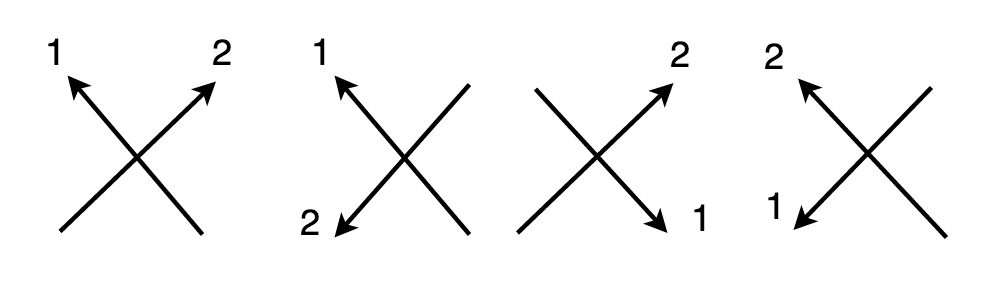
\includegraphics[width=\textwidth]{dollarnstrokes}
\caption[Examples of stroke permutations]{Some permutations possible for an 'X'. The numbers represent the order in which they are drawn, and the arrow represents the direction of the stroke.}
\label{fig:nstrokes}
\end{figure}

The \$N uses the same processes as the \$1, except on multiple strokes. The main challenge of multistrokes is that any of the strokes can be drawn in any order and from any direction. As shown in Figure \ref{fig:nstrokes}, even a simple two stroke gesture has multiple combinations. The \$N recognizer orders the points in each possible permutation - essentially treating each multistroke permutation as a unistroke. A Heap Permute is used to generate all possible permutations of strokes \cite{dollarN}. The \$N also operates with bounded rotational invariance, meaning an object flipped completely upside down (rotated 180 degrees) will be recognized as a completely different gesture. The bounds for rotation are set to $\pm$ 90 $^{\circ}$.  These permutations are generated for each template, then compared to the user input. The one with the lowest score (smallest difference) is chosen as the classification for the user input. \\

During the initial development of this work, I relied heavily on the \$N recognizer to recognize all objects in the system. However, it failed to accurately classify different combinations of strokes too often. The exhaustion of all permutations of combinations of strokes meant that it more often than not found connections between combinations of strokes the user did not intend. While it may have been possible to more intelligently select combinations of strokes to classify, it became apparent that this tool was far too flexible for our needs. In chapter 3, we will discuss our replacement solution for this recognizer and how we overcame these issues.

\section{Related Software}

This work shares qualities and goals with other sketching software. Two such examples are Lightsketch created by Glaser \textit{et. al} \cite{glaser2003sketch} and Yi-Luen Do's VRSketchpad \cite{do2001vr}, both of which are also architectural sketching interfaces. LightSketch is similar to OASIS and uses sketching vocabulary \cite{glaser2003sketch} similar to the new sketching interface. In particular, LightSketch also shares a `sketch-based` interface with a minimal user interface. Similar to this sketching interface, LightSketch can also recognize shapes shapes and symbols. However, Lightsketch does not have any shape indications or overlaid shapes to indicate to the user the interface's intent. Also, LightSketch does not appear to have any methods of editing previously drawn primitives, while this sketching interface allows users to change, edit and reclassify previously created lines. \\

VRSketchpad also employs a freehand sketch approach to their interface. Similar to our implementation, VRSketchpad processes the user design and translates the drawings into 3D objects. VRSketchpad also has multiple levels to processing to create shapes, irregular shapes, and pieces of furniture. However, VRSketchpad contains a much busier interface than our own, which is devoid of buttons and modes. Unlike our implementation, VRSketchpad has no recognition before processing the drawing into a 3D model. Therefore, we can give the user a better idea of our interpretation of his/her design before creating the 3D model.\\

% Rubine's specifying gestures by example
% SATIN
One example of a non-architectural sketching interface is the Gesture Recognizers Automated in a Novel Direct Manipulation Architecture (GRANDMA) created by Rubine. Rubine describes a series of features that are incrementally computable in constant time per input \cite{rubinegestures}. These features include cosine and sin of the initial angle of the stroke, duration of the strokes, bound box diagonal of the stroke, and distance of the stroke in total. These features are also used in other applications, such as SATIN, a toolkit for informal ink-based applications \cite{satin}. In order to classify strokes, weights were attached to features depending on their importance to that classification. Rubine's system also had the ability to reject classification if the gesture was deemed ambiguous or if it was not confident in its recognition. When a user created stroke was run against a template, the highest scoring classification would be applied. These features were applied to create his gesture-based drawing program (GDP). GDP was a simple drawing program with robust features by drawing unistroke commands to specify certain actions. For example, a user could use the `delete` command, and the next unistroke would be executed as a delete command. Our implementation uses a similar system when attempting to classify rectangles. Also, both interfaces use a minimal interface, relying solely on user drawn strokes. However, Rubine's implementation uses a training set to learn the unistrokes recognized by the program, while my implementation does not require the use of any training data. In chapter 4, we will discuss further in depth the features chosen to represent our objects. \\

\section{Summary}
This chapter provides an overview of the works that influenced the design and development of this project. The previous feature development on the OASIS system helped to develop an interface suitable for OASIS itself. As we will discuss in chapter 3, many of the technologies used in OASIS will also be used to develop this work. Different works in human input recognition led me to choose a geometric based approach to classifying user strokes. This work will provide an enhanced user experience when designing models on OASIS.